\documentclass[aspectratio=169]{beamer}
\usetheme{Madrid}
\usepackage[utf8]{inputenc}
\usepackage[T1]{fontenc}
\usepackage{tikz}
\usepackage{amssymb}
\usepackage{graphicx}
\setbeamertemplate{navigation symbols}{}
\setbeamercolor{title}{fg=white,bg=green!55!teal}
\setbeamercolor{frametitle}{fg=white,bg=green!55!teal}
\setbeamercolor{block title}{bg=green!55!teal!20,fg=black}
\setbeamercolor{block body}{bg=green!55!teal!8,fg=black}
\setbeamercolor{item}{fg=green!55!teal}
\setbeamercolor{itemize item}{fg=green!55!teal}
\setbeamertemplate{itemize item}[triangle]

\title{M2 — Choices \& Loops}
\subtitle{if/elif/else, while, for-range — predict the drawing before you run it}
\author{ByteForge --- Grade 8 --- App Builder}
\date{}

\begin{document}

\begin{frame}
    \titlepage
\end{frame}

\begin{frame}{Today's Plan}
    \begin{itemize}
        \item Odd or Even
        \item FizzBuzz Lite
        \item Countdown Circles
        \item Grade Classifier
        \item Sum to N
        \item[$\bigstar$] BOSS --- M2 Capstone
    \end{itemize}
\end{frame}

\begin{frame}{if/else — real syntax for a decision}
    \large
    \begin{itemize}
        \item \texttt{number \% 2} gives what's LEFT OVER after dividing by 2
        \item 0 for even, 1 for odd. The exact same MOD idea from Grade 7, just written as \texttt{\%}.
    \end{itemize}

    \begin{center}
    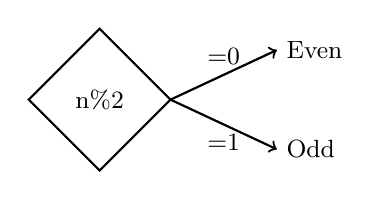
\begin{tikzpicture}[scale=0.9]

        \draw[thick] (1,1) -- (2,0) -- (1,-1) -- (0,0) -- cycle;
        \node at (1,0) {\small n\%2};
        \draw[->, thick] (2,0) -- (3.5,0.7) node[midway,above]{\small =0};
        \node[right] at (3.5,0.7) {\small Even};
        \draw[->, thick] (2,0) -- (3.5,-0.7) node[midway,below]{\small =1};
        \node[right] at (3.5,-0.7) {\small Odd};
    \end{tikzpicture}
    \end{center}
\end{frame}


\begin{frame}{for loops with range(), and elif chains}
    \large
    \begin{itemize}
        \item \texttt{for i in range(1, 11):} loops through 1 to 10
        \item The second number is EXCLUSIVE, which is why you need 11 to reach 10. This trips up almost everyone the first time.
    \end{itemize}
\end{frame}


\begin{frame}{while loops — repeat until a condition is false}
    \large
    \begin{itemize}
        \item \texttt{for} is perfect when you know the count in advance. \texttt{while size > 0:} keeps going for as long as a CONDITION stays true
        \item The loop MUST change the condition eventually, or it runs forever.
    \end{itemize}
\end{frame}


\begin{frame}{Chained if/elif — order decides correctness}
    \large
    \begin{itemize}
        \item Checking \texttt{>= 70} BEFORE \texttt{>= 90} would wrongly grade a 95 as a "B"
        \item Order in a chain of conditions genuinely changes the result.
    \end{itemize}
\end{frame}

\begin{frame}{Real-World Examples}
    \large
    \begin{itemize}
        \item Every "off by one" range bug (\texttt{range(1,11)} needing 11, not 10) is a genuinely common real bug professional developers still make. Minecraft's own farming/breeding cooldowns are \texttt{while} loops in disguise
        \item "keep waiting while the cooldown timer is still above zero".
    \end{itemize}
\end{frame}


\begin{frame}{Image}
    \begin{center}
    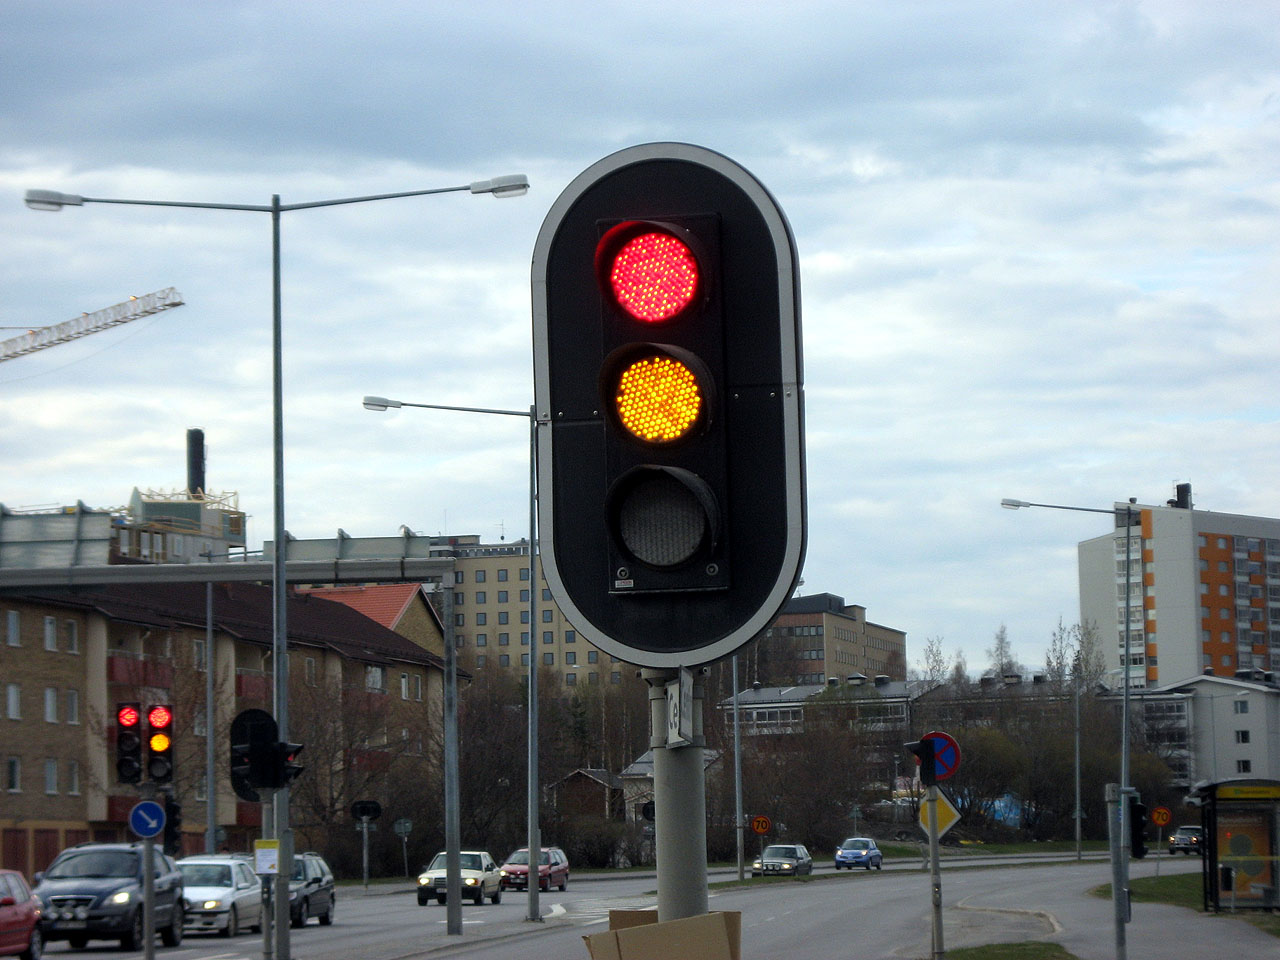
\includegraphics[width=0.5\textwidth]{images/traffic.jpg}

    \large A real three-way branch --- the same if/elif/else idea from this chapter.

    \small LED traffic lights, public domain (PD-self), via Wikimedia Commons
    \end{center}
\end{frame}

\begin{frame}{Let Them Discover}
    \Large
    Before running anything: what does \texttt{range(1, 11)} actually produce — does it include 11? Write your guess down, then check — this exact mistake is one of the most common real beginner bugs.
\end{frame}

\begin{frame}{Your Turn}
    \Large
    Open the student map, find \textbf{M2 — Choices \& Loops}, and work through it
    hands-on --- everything you just saw, they now do themselves.
\end{frame}

\end{document}
